\subsection{Punto de Vista de la Aplicación}
El punto de vista de Aplicación describe el comportamiento interno de una aplicación; por ejemplo, cuando realiza uno o más servicios de aplicación.

\subsubsection{Punto de Vista de comportamiento}
Este punto de vista es útil para diseñar el comportamiento principal de las aplicaciones o para identificar la superposición funcional entre diferentes aplicaciones. Se preocupa por la estructura, relaciones y dependencias entre aplicaciones, consistencia e integridad, reducción de complejidad de la aplicación
\begin{figure}[th!]
	\centering
	\fcolorbox{black}{white}{
		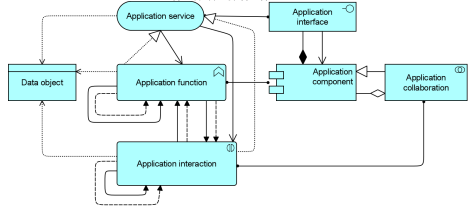
\includegraphics[width=0.9\linewidth]{imgs/puntos_vista/aplicacion/vistacomportamiento}}
	\caption{vista de comportamiento de aplicación}
	\label{fig:vistaaplicacion}
\end{figure}

\subsubsection{Punto de Vista de cooperacion}
El punto de vista de la cooperación de aplicaciones describe las relaciones entre los componentes de las aplicaciones en términos de los flujos de información entre ellos, o en términos de los servicios que ofrecen y utilizan. Este punto de vista se utiliza normalmente para crear una descripción general del panorama de aplicaciones de una organización. Este punto de vista también se utiliza para expresar la cooperación interna o la orquestación de servicios que en conjunto apoyan la ejecución de un proceso empresarial.

\begin{figure}[th!]
	\centering
	\fcolorbox{black}{white}{
		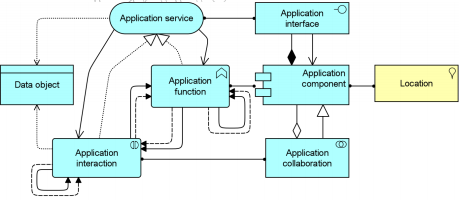
\includegraphics[width=0.9\linewidth]{imgs/puntos_vista/aplicacion/vistacooperacion}}
	\caption{vista de cooperacion de aplicación}
	\label{fig:vistaaplicacion}
\end{figure}

\subsubsection{Punto de Vista de estructura}
El punto de vista Estructura de la aplicación muestra la estructura de una o más aplicaciones o componentes. 
Este punto de vista es útil para diseñar o comprender la estructura principal de aplicaciones o componentes y los datos asociados; p. ej., para desglosar la estructura del sistema en construcción o para identificar componentes de aplicaciones heredados que son adecuados para la migración / integración
\begin{figure}[th!]
	\centering
	\fcolorbox{black}{white}{
		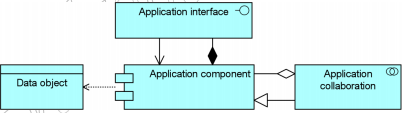
\includegraphics[width=0.9\linewidth]{imgs/puntos_vista/aplicacion/vistaestructura}}
	\caption{vista de estructura de aplicación}
	\label{fig:vistaaplicacion}
\end{figure}	

\subsubsection{Punto de Vista de uso}
El punto de vista Uso de aplicaciones describe cómo se utilizan las aplicaciones para dar soporte a uno o más procesos de negocio y cómo las utilizan otras aplicaciones. 
Se puede utilizar para diseñar una aplicación identificando los servicios que necesitan los procesos de negocio y otras aplicaciones, o para diseñar procesos de negocio al describir los servicios que están disponibles. 